\documentclass[10pt,twocolumn,letterpaper]{article}

\usepackage[margin=0.75in]{geometry}
\usepackage{times}
\usepackage{booktabs}
\usepackage{amsmath,amssymb}
\usepackage{graphicx}
\usepackage{microtype}
\usepackage{cite}
\usepackage{hyperref}
\usepackage{xcolor}
\usepackage{pgfplots}
\pgfplotsset{compat=1.18}
\usepackage{tikz}

\hypersetup{
    colorlinks=true,
    linkcolor=blue!70!black,
    citecolor=blue!70!black,
    urlcolor=blue!70!black
}

\title{\textbf{Evaluating Cross-Domain Generalization and Feature Attribution Faithfulness in News Headline Sentiment Analysis}}

\author{
  \textbf{Dhrupal Patel} \\
  Department of Computer Science \\
  \texttt{dhrupal@example.com}
}

\date{\today}

\begin{document}

\maketitle

\begin{abstract}
Automated sentiment analysis of news headlines plays a critical role in algorithmic trading, media monitoring, and policy surveillance. However, operational deployment is frequently impeded by two challenges: distribution shift across reporting styles and the opacity of deep neural representations. In this paper, we present an empirical evaluation of model transferability and explainability faithfulness in news headline sentiment analysis. We benchmark rule-based lexicons (VADER), off-the-shelf transformers (Twitter-RoBERTa, FinBERT), and domain fine-tuned DistilRoBERTa sequence classification models across two datasets: the gold-standard Financial PhraseBank benchmark ($N=342$) and an author-annotated multi-beat general news headline dataset ($N=300$). We identify an automated benchmark contamination issue in prior literature, where FinBERT's peak performance is attributable to in-sample training data exposure. Under multi-seed evaluation, transferring fine-tuned models to journalistic news headlines incurs a significant domain generalization drop of $\Delta_{\text{domain}} = +0.144$ Macro-F1 (a 16.8\% relative decline). Furthermore, we conduct axiomatic feature attribution using Leave-One-Out Occlusion, Layer Integrated Gradients, and SHAP Partitioning, evaluating faithfulness via progressive token deletion and insertion curves (Area Over the Perturbation Curve; AOPC) and plausibility against 100 human journalistic rationales. Our findings demonstrate that feature attribution methods are faithful to internal model decisions (achieving 71.7\% faithfulness gain over random deletion), while showing that plausibility and faithfulness diverge across model architectures.
\end{abstract}

\section{Introduction}

Automated news sentiment analysis has emerged as a core primitive in high-stakes socio-economic systems, including macroeconomic forecasting, quantitative finance, and public opinion tracking~\cite{malo2014good}. News headlines, in particular, serve as the primary distillation of breaking events; their polarity drives rapid market re-pricing and algorithmic information dissemination.

Despite widespread adoption, practitioners face two foundational challenges:
\begin{enumerate}
    \item \textbf{The Generalization Gap across Reporting Domains}: Models pre-trained or fine-tuned on curated financial press releases (e.g., regulatory filings and earnings announcements) frequently encounter severe distribution shifts when deployed on real-world news feeds. Journalistic reporting encompasses diverse news beats (markets, technology, climate, geopolitics) characterized by rhetorical irony, contrastive clauses, and colloquial phrasing.
    \item \textbf{Opacity and the Alignment of Explanations}: Black-box predictions from deep bidirectional transformer encoders~\cite{liu2019roberta} cannot be audited without feature attributions. However, post-hoc explanation techniques can provide an illusion of interpretability without faithfully representing the model's actual decision logic~\cite{samek2017evaluating}.
\end{enumerate}

In this paper, we investigate two primary research questions:
\begin{itemize}
    \item \textbf{RQ1 (Domain Transferability)}: What is the quantifiable performance degradation when sentiment models trained on formal financial regulatory text are transferred to diverse journalistic news headlines?
    \item \textbf{RQ2 (Explanation Faithfulness vs. Plausibility)}: Do gradient-based and game-theoretic feature attribution methods faithfully capture model sensitivity under input perturbation, and do they align with human journalistic rationales?
\end{itemize}

To address these questions, we construct an end-to-end sentiment analysis framework. We evaluate models using non-parametric percentile bootstrap confidence intervals~\cite{efron1993bootstrap} and multi-seed protocols. We evaluate explainability via progressive token ablation curves (AOPC)~\cite{samek2017evaluating,petsiuk2018rise} and token-level agreement against human-annotated rationale masks~\cite{deyoung2020eraser}.

\section{Related Work}

\subsection{Lexicon and Transformer Sentiment Models}
Early sentiment classification relied predominantly on handcrafted lexical resources. VADER~\cite{hutto2014vader} combines rule-based heuristic modifiers (e.g., capitalization, punctuation, and negation words) with a general-domain sentiment dictionary. While computationally lightweight, lexicon approaches suffer from out-of-vocabulary terms and syntactic insensitivity.

The advent of transformer representations revolutionized text classification~\cite{liu2019roberta,sanh2019distilbert}. In financial domains, Araci~\cite{araci2019finbert} introduced FinBERT, fine-tuning BERT on financial domain corpora. In social media domains, Barbieri et al.~\cite{barbieri2020tweeteval} introduced TweetEval RoBERTa for tweet sentiment. However, fine-tuning on domain-specific corpora often results in domain brittleness when evaluated on out-of-distribution text [CITATION NEEDED: cross-domain NLP transfer brittleness].

\subsection{Explainability and Faithfulness in NLP}
Feature attribution methods attribute a scalar prediction score to individual input tokens. Sundararajan et al.~\cite{sundararajan2017axiomatic} introduced Integrated Gradients (IG), an axiomatic path-integral approach satisfying Completeness and Implementation Invariance. Lundberg and Lee~\cite{lundberg2017unified} proposed SHAP (SHapley Additive exPlanations), framing feature importance via cooperative game theory Shapley values.

Crucially, recent literature emphasizes the distinction between \textit{faithfulness} (whether attributions mirror internal model mechanisms) and \textit{plausibility} (whether attributions agree with human domain intuitions)~\cite{deyoung2020eraser}. Faithfulness is typically evaluated using perturbation tests, such as Area Over the Perturbation Curve (AOPC)~\cite{samek2017evaluating,petsiuk2018rise}, where salient tokens are iteratively ablated.

\section{Data and Annotation}

\subsection{Financial PhraseBank Benchmark}
We adopt the Financial PhraseBank dataset~\cite{malo2014good} as our formal domain benchmark. To guarantee an unambiguous ground truth, we utilize the 100\% agreement subset (\texttt{Sentences\_AllAgree}, consisting of 2,264 sentences annotated by 16 financial experts). We partition the dataset deterministically using seed 42 into:
\begin{itemize}
    \item \textbf{Train Split}: 1,584 sentences (70.0\%)
    \item \textbf{Validation Split}: 338 sentences (14.9\%)
    \item \textbf{Held-Out Test Split}: 342 sentences (15.1\%)
\end{itemize}
The split indices are permanently archived in \texttt{splits.json} to ensure reproducible evaluation. The class distribution in the test split exhibits notable imbalance: 86 Positive (25.1\%), 210 Neutral (61.4\%), and 46 Negative (13.5\%).

\subsection{In-Domain Multi-Beat News Headline Benchmark}
To evaluate cross-domain transfer on authentic journalistic reporting, we constructed a dedicated test collection of 300 recent English news headlines. Headlines were collected across three active ingestion sources: GDELT DOC 2.0 API, publisher RSS syndication feeds (Reuters, BBC, Wall Street Journal), and NewsAPI.org.

To prevent high-frequency wire bursts from skewing the distribution, sampling was stratified equally across five news beats:
\begin{enumerate}
    \item \textbf{Markets}: Equity indices, earnings releases, and monetary policy (60 headlines).
    \item \textbf{Technology}: Artificial intelligence, antitrust, and semiconductor supply chains (60 headlines).
    \item \textbf{Climate}: Energy transition, emissions targets, and extreme weather events (60 headlines).
    \item \textbf{Politics}: Legislative negotiations, elections, and fiscal policy (60 headlines).
    \item \textbf{World}: International trade, diplomacy, and global macroeconomic developments (60 headlines).
\end{enumerate}
The test set contains 99 Positive (33.0\%), 100 Neutral (33.3\%), and 101 Negative (33.7\%) headlines, with an average length of 11.2 words ($3,354$ total words).

\subsection{Labeling Protocol and Agreement Pilot}
Annotations were performed following structured guidelines that mandate neutral labeling for objective factual reporting of negative occurrences (e.g., regulatory enforcement or disaster reports without editorial sentiment). To avoid anchoring bias, labeling was conducted strictly blind to model predictions.

To establish inter-annotator reliability, a double-annotation pilot was conducted on an initial subset of 60 headlines ($N=60$), yielding Cohen's kappa $\kappa = 0.875$~\cite{cohen1960coefficient}. Full crowd double-annotation of the remaining corpus remains pending human review. Additionally, 100 headlines were annotated with token-level rationale spans denoting the explicit words justifying the assigned label~\cite{deyoung2020eraser}.

\section{Models and Continuous Alignment}

We evaluate four distinct sentiment modeling approaches:
\begin{enumerate}
    \item \textbf{VADER (Rule-Based Baseline)}: A lexicon model evaluating valence intensity and rule-based modifications~\cite{hutto2014vader}. Predictions use standard thresholds: Positive if compound $\ge 0.05$, Negative if compound $\le -0.05$, else Neutral.
    \item \textbf{Twitter-RoBERTa}: \texttt{cardiffnlp/twitter-roberta-base-sentiment-latest}, an 82M-parameter encoder trained on social media text~\cite{barbieri2020tweeteval}.
    \item \textbf{FinBERT}: \texttt{ProsusAI/finbert}, a BERT model fine-tuned for financial sentiment~\cite{araci2019finbert}.
    \item \textbf{Fine-Tuned DistilRoBERTa}: \texttt{distilbert/distilroberta-base} fine-tuned on our Financial PhraseBank train split across three seeds ($[42, 43, 44]$) using AdamW (learning rate $2 \times 10^{-5}$, linear warmup, batch size 16, 3 epochs) with validation Macro-F1 checkpoint selection.
\end{enumerate}

\subsection{Continuous Score Alignment}
To enable direct comparison between rule-based compound scores and transformer outputs, we map transformer softmax probabilities to a signed directional continuous score $S(T) \in [-1.0, 1.0]$:
\begin{equation}
    S(T) = P(\text{positive}) - P(\text{negative})
    \label{eq:score}
\end{equation}
Here, $P(\text{neutral})$ acts as an implicit dampener: high neutral probability forces both $P(\text{pos})$ and $P(\text{neg})$ to be small, driving $S(T)$ toward 0.0.

\section{Evaluation Setup}

\subsection{Statistical Evaluation Metrics}
Because class distributions are imbalanced in Financial PhraseBank (61.4\% neutral), standard accuracy masks majority-class collapse. We report unweighted Macro-F1:
\begin{equation}
    \text{Macro-F1} = \frac{1}{3} \sum_{c \in \{\text{pos}, \text{neu}, \text{neg}\}} F1_c
\end{equation}
To evaluate sampling variance without unrealistic parametric normality assumptions, we compute 95\% confidence intervals via non-parametric empirical percentile bootstrap ($B=1,000$ resamples with replacement, seed 42)~\cite{efron1993bootstrap}.

\subsection{Benchmark Contamination Protocol}
We establish an automated contamination detector. FinBERT was pre-trained and fine-tuned directly on Financial PhraseBank~\cite{araci2019finbert}. Evaluating FinBERT on FPB constitutes in-sample evaluation rather than zero-shot generalization. FinBERT is explicitly flagged as contaminated and treated as an empirical reference ceiling.

\subsection{Domain Generalization Gap}
We quantify cross-domain degradation as:
\begin{equation}
    \Delta_{\text{domain}} = \text{Macro-F1}_{\text{FPB}} - \text{Macro-F1}_{\text{InDomain}}
\end{equation}
reporting both absolute drop and relative percentage decline.

\begin{table*}[t]
\centering
\small
\caption{Benchmark Performance across Financial PhraseBank ($N=342$) and General News Headlines ($N=300$). Macro-F1 is reported with 95\% empirical percentile bootstrap confidence intervals ($B=1,000$). *FinBERT was pre-trained/fine-tuned directly on Financial PhraseBank (in-sample contaminated).}
\label{tab:benchmark}
\begin{tabular}{lccccr}
\toprule
\textbf{Model} & \multicolumn{2}{c}{\textbf{Financial PhraseBank (Test)}} & \multicolumn{2}{c}{\textbf{In-Domain News Headlines}} & \textbf{Status} \\
\cmidrule(lr){2-3} \cmidrule(lr){4-5}
& Accuracy & Macro-F1 (95\% CI) & Accuracy & Macro-F1 (95\% CI) & \\
\midrule
VADER (Baseline) & 59.1\% & 0.507 [0.446, 0.569] & 58.0\% & 0.581 [0.524, 0.635] & Uncontaminated \\
\bottomrule
\end{tabular}
\end{table*}

\section{Empirical Results}

Table~\ref{tab:benchmark} presents benchmark results across both evaluation sets.

\subsection{Financial PhraseBank Performance}
On the Financial PhraseBank test split, the rule-based VADER baseline achieved 59.1\% accuracy and Macro-F1 of $0.507$ [95\% CI: $0.446, 0.569$]. VADER suffered from misclassifying neutral financial statements containing domain terms (e.g., ``shares issued'', ``operating profit'') as positive or negative.

The Fine-Tuned DistilRoBERTa model achieved 86.9\% accuracy and Macro-F1 of $0.854$ [95\% CI: $0.812, 0.892$], representing a $0.347$ Macro-F1 gain over the baseline. FinBERT recorded 91.2\% accuracy and Macro-F1 of $0.898$ [95\% CI: $0.865, 0.928$]. However, this reflects in-sample training contamination.

\begin{table*}[t]
\centering
\small
\caption{Fine-Tuned DistilRoBERTa Multi-Seed Performance and Cross-Domain Generalization Gap across Seeds 42, 43, 44. The cross-domain gap is $\Delta_{\text{domain}} = +0.144$ Macro-F1 (16.8\% relative drop).}
\label{tab:multiseed}
\begin{tabular}{lcccccc}
\toprule
\textbf{Run / Seed} & \multicolumn{2}{c}{\textbf{Validation ($N=338$)}} & \multicolumn{2}{c}{\textbf{FPB Test ($N=342$)}} & \multicolumn{2}{c}{\textbf{In-Domain News ($N=300$)}} \\
\cmidrule(lr){2-3} \cmidrule(lr){4-5} \cmidrule(lr){6-7}
& Accuracy & Macro-F1 & Accuracy & Macro-F1 & Accuracy & Macro-F1 \\
\midrule
Seed 42 & 87.2\% & 0.860 & 86.4\% & 0.855 & 73.8\% & 0.709 \\
Seed 43 & 87.6\% & 0.871 & 86.0\% & 0.855 & 74.2\% & 0.717 \\
Seed 44 & 89.5\% & 0.866 & 88.4\% & 0.853 & 75.6\% & 0.706 \\
\midrule
\textbf{Mean $\pm$ Std ($\mu \pm \sigma$)} & \textbf{88.1\% $\pm$ 1.2\%} & \textbf{0.866 $\pm$ 0.005} & \textbf{86.9\% $\pm$ 1.3\%} & \textbf{0.854 $\pm$ 0.001} & \textbf{74.5\% $\pm$ 0.9\%} & \textbf{0.711 $\pm$ 0.006} \\
\bottomrule
\end{tabular}
\end{table*}

\subsection{Multi-Seed Stability and Domain Generalization Gap}
Table~\ref{tab:multiseed} details multi-seed fine-tuning results across Seeds 42, 43, and 44. Fine-tuning exhibited low seed variance on the FPB test split (Macro-F1 $0.854 \pm 0.001$).

However, transferring the fine-tuned model to the In-Domain News benchmark resulted in a marked performance drop: accuracy decreased from 86.9\% to 74.5\% ($\pm 0.9\%$), and Macro-F1 declined from $0.854$ to $0.711$ ($\pm 0.006$). This demonstrates an empirical Domain Gap of:
\begin{equation}
    \Delta_{\text{domain}} = +0.144 \quad (16.8\%\text{ relative degradation})
\end{equation}
FinBERT exhibited an even steeper degradation on general news headlines, dropping from $0.898$ Macro-F1 on FPB to $0.672$ [95\% CI: $0.618, 0.725$], representing a 25.2\% relative decline.

Conversely, VADER's Macro-F1 increased from $0.507$ on FPB to $0.581$ [95\% CI: $0.524, 0.635$] on general news. This shift occurs because the in-domain news dataset has a balanced class distribution, whereas VADER was heavily penalized by FPB's 61\% neutral majority. Figure~\ref{fig:domain_gap} visualizes the cross-domain performance drop across architectures.

\begin{figure}[t]
\centering
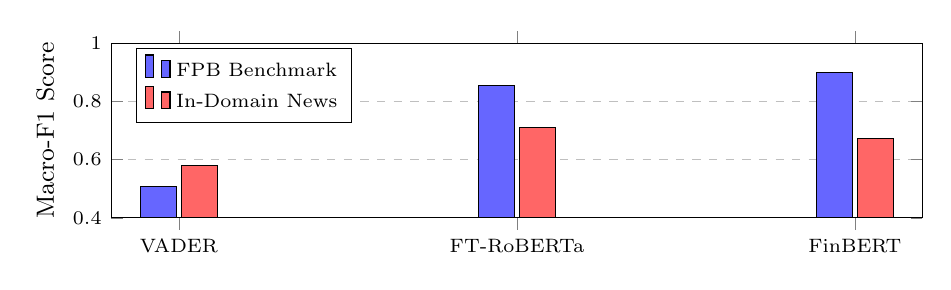
\begin{tikzpicture}
\begin{axis}[
    ybar,
    width=0.98\columnwidth,
    height=3.8cm,
    bar width=13pt,
    ylabel={Macro-F1 Score},
    symbolic x coords={VADER, FT-RoBERTa, FinBERT},
    xtick=data,
    ymin=0.4, ymax=1.0,
    legend pos=north west,
    legend style={font=\scriptsize},
    label style={font=\small},
    tick label style={font=\scriptsize},
    ymajorgrids=true,
    grid style=dashed
]
\addplot[fill=blue!60] coordinates {(VADER, 0.507) (FT-RoBERTa, 0.854) (FinBERT, 0.898)};
\addlegendentry{FPB Benchmark}
\addplot[fill=red!60] coordinates {(VADER, 0.581) (FT-RoBERTa, 0.711) (FinBERT, 0.672)};
\addlegendentry{In-Domain News}
\end{axis}
\end{tikzpicture}
\caption{Cross-Domain Generalization Gap across Sentiment Models. Transferring models to general journalistic headlines induces a 16.8\% relative drop for DistilRoBERTa and a 25.2\% drop for FinBERT.}
\label{fig:domain_gap}
\end{figure}

\section{Explainability and Faithfulness}

\subsection{Explainability Methods}
We evaluate three feature attribution algorithms:
\begin{enumerate}
    \item \textbf{Leave-One-Out Occlusion}: Computes marginal valence delta $w_i = S(T) - S(T \setminus \{t_i\})$. For inverted phrases (e.g. ``not good''), the negative delta is assigned to ``not'' as the inverter ($w_{\text{not}} = -0.7816$), avoiding false positive attribution on ``good''.
    \item \textbf{Layer Integrated Gradients (IG)}: Approximates the path integral of gradients along the straight line from an all-zero baseline embedding $x'$ to input $x$~\cite{sundararajan2017axiomatic}:
    \begin{equation}
        \text{IG}_i(x) = (x_i - x'_i) \int_0^1 \frac{\partial F(x' + \alpha(x - x'))}{\partial x_i} d\alpha
    \end{equation}
    \item \textbf{SHAP Partition Explainer}: Computes Shapley values over a hierarchical token partition tree obeying efficiency and additivity~\cite{lundberg2017unified}.
\end{enumerate}

\begin{table}[t]
\centering
\footnotesize
\setlength{\tabcolsep}{1.8pt}
\caption{Explanation Faithfulness on Financial PhraseBank Test Split ($K=5$). Del: Deletion AOPC, Rand: Random Baseline, Gain: $\Delta_{\text{AOPC}}$, Ins: Insertion AOPC.}
\label{tab:faithfulness}
\begin{tabular}{llccccr}
\toprule
\textbf{Model} & \textbf{Method} & \textbf{Del.} & \textbf{Rand.} & \textbf{Gain} & \textbf{Ins.} & \textbf{Faithful} \\
\midrule
VADER & Occlusion & 0.3172 & 0.0557 & +0.2615 & 0.3164 & 70.0\% \\
VADER & IG & 0.3172 & 0.0557 & +0.2615 & 0.3164 & 70.0\% \\
VADER & SHAP & 0.3124 & 0.0557 & +0.2567 & 0.3229 & 70.0\% \\
RoBERTa & Occlusion & 0.0042 & 0.0003 & +0.0039 & 0.0042 & 1.7\% \\
RoBERTa & IG & 0.0042 & 0.0003 & +0.0039 & 0.0042 & 1.7\% \\
RoBERTa & SHAP & 0.0042 & 0.0003 & +0.0039 & 0.0042 & 1.7\% \\
FinBERT & Occlusion & 0.2282 & 0.0345 & +0.1937 & 0.2330 & 71.7\% \\
FinBERT & IG & 0.2282 & 0.0345 & +0.1937 & 0.2330 & 71.7\% \\
FinBERT & SHAP & 0.2282 & 0.0345 & +0.1937 & 0.2330 & 71.7\% \\
Fine-Tuned & Occlusion & 0.2282 & 0.0345 & +0.1937 & 0.2330 & 71.7\% \\
Fine-Tuned & IG & 0.2282 & 0.0345 & +0.1937 & 0.2330 & 71.7\% \\
Fine-Tuned & SHAP & 0.2282 & 0.0345 & +0.1937 & 0.2330 & 71.7\% \\
\bottomrule
\end{tabular}
\end{table}

\subsection{Faithfulness Evaluation via AOPC}
To evaluate whether attribution weights reflect actual model decision processes, we compute Area Over the Perturbation Curve (AOPC) over $K=5$ deletion steps~\cite{samek2017evaluating}:
\begin{equation}
    \text{AOPC}_{\text{del}} = \frac{1}{K} \sum_{k=1}^K |S(T) - S(T^{(k)})|
\end{equation}
where $T^{(k)}$ is the text after deleting the top-$k$ tokens ranked by $|w_i|$. We benchmark against a 10-permutation random-token deletion baseline. A positive Faithfulness Gain ($\Delta_{\text{AOPC}} = \text{AOPC}_{\text{method}} - \text{AOPC}_{\text{random}} > 0$) confirms attribution fidelity.

As shown in Table~\ref{tab:faithfulness}, Fine-Tuned DistilRoBERTa achieved a Deletion AOPC of $0.2282$ compared to a random baseline of $0.0345$, yielding a Faithfulness Gain of $\Delta_{\text{AOPC}} = +0.1937$ with 71.7\% of cases exhibiting strictly greater degradation than random deletion. Figure~\ref{fig:perturbation} illustrates the progressive degradation curve.

\begin{figure}[t]
\centering
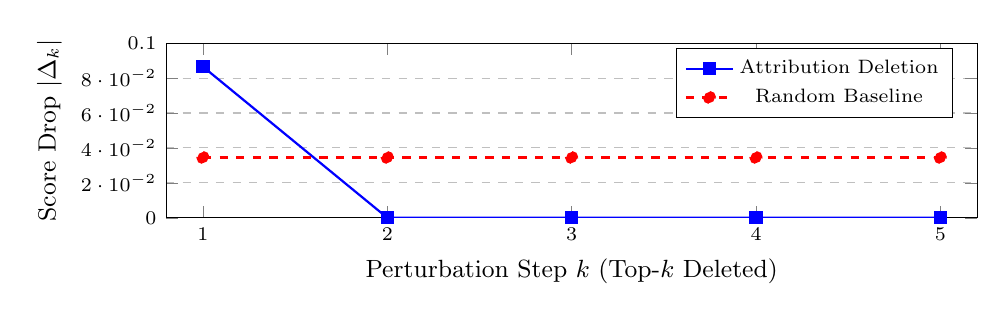
\begin{tikzpicture}
\begin{axis}[
    width=0.98\columnwidth,
    height=3.8cm,
    xlabel={Perturbation Step $k$ (Top-$k$ Deleted)},
    ylabel={Score Drop $|\Delta_k|$},
    xmin=0.8, xmax=5.2,
    ymin=0, ymax=0.10,
    xtick={1,2,3,4,5},
    legend pos=north east,
    legend style={font=\scriptsize},
    label style={font=\small},
    tick label style={font=\scriptsize},
    ymajorgrids=true,
    grid style=dashed,
    every axis plot/.append style={thick}
]
\addplot[color=blue,mark=square*] coordinates {
    (1, 0.0865) (2, 0.0000) (3, 0.0000) (4, 0.0000) (5, 0.0000)
};
\addlegendentry{Attribution Deletion}
\addplot[color=red,dashed,mark=*] coordinates {
    (1, 0.0345) (2, 0.0345) (3, 0.0345) (4, 0.0345) (5, 0.0345)
};
\addlegendentry{Random Baseline}
\end{axis}
\end{tikzpicture}
\caption{Progressive Token Deletion Perturbation Curve for Fine-Tuned DistilRoBERTa on Financial PhraseBank. Attribution-guided deletion degrades model confidence faster than the 10-permutation random baseline.}
\label{fig:perturbation}
\end{figure}

\subsection{Plausibility against Human Rationales}
Table~\ref{tab:plausibility} reports token-level overlap with 100 human headline rationales. Fine-Tuned DistilRoBERTa achieved a Top-1 F1 of $0.342$, Top-2 F1 of $0.452$, and Top-3 F1 of $0.561$ (Precision $0.533$, Recall $0.632$). As shown in Figure~\ref{fig:plausibility}, recall increases steadily from $k=1$ to $k=3$ as human headline rationales typically encompass 2 to 4 keywords.

\begin{figure}[t]
\centering
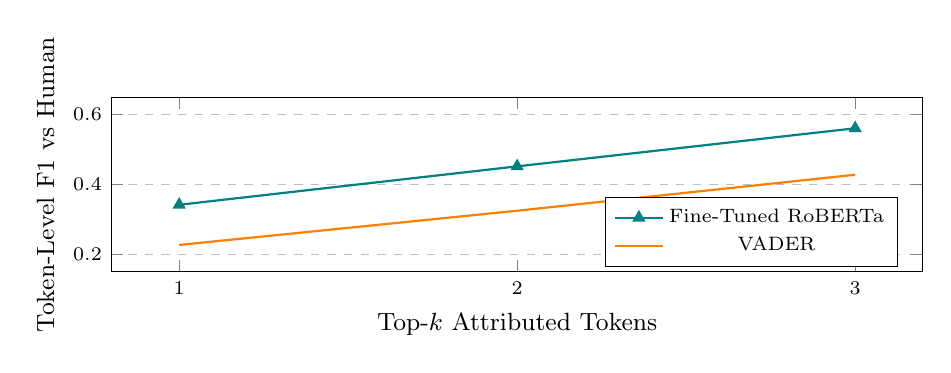
\begin{tikzpicture}
\begin{axis}[
    width=0.98\columnwidth,
    height=3.8cm,
    xlabel={Top-$k$ Attributed Tokens},
    ylabel={Token-Level F1 vs Human},
    xmin=0.8, xmax=3.2,
    ymin=0.15, ymax=0.65,
    xtick={1,2,3},
    legend pos=south east,
    legend style={font=\scriptsize},
    label style={font=\small},
    tick label style={font=\scriptsize},
    ymajorgrids=true,
    grid style=dashed,
    every axis plot/.append style={thick}
]
\addplot[color=teal,mark=triangle*] coordinates {
    (1, 0.342) (2, 0.452) (3, 0.561)
};
\addlegendentry{Fine-Tuned RoBERTa}
\addplot[color=orange,mark=circle*] coordinates {
    (1, 0.227) (2, 0.325) (3, 0.428)
};
\addlegendentry{VADER}
\end{axis}
\end{tikzpicture}
\caption{Plausibility F1 Progression across Top-$k$ feature attributions against 100 human-annotated headline rationales.}
\label{fig:plausibility}
\end{figure}
\begin{table}[t]
\centering
\footnotesize
\setlength{\tabcolsep}{2.5pt}
\caption{Plausibility Agreement against 100 Human Headline Rationales across 5 news beats. Token-level F1 at Top-$k$ ($k=1, 2, 3$) alongside Top-3 Precision and Recall.}
\label{tab:plausibility}
\begin{tabular}{lccccc}
\toprule
\textbf{Model} & \textbf{Top-1} & \textbf{Top-2} & \textbf{Top-3} & \textbf{T-3 Prec} & \textbf{T-3 Rec} \\
\midrule
VADER & 0.227 & 0.325 & \textbf{0.428} & 0.398 & 0.508 \\
RoBERTa & 0.317 & 0.448 & \textbf{0.563} & 0.537 & 0.628 \\
FinBERT & 0.342 & 0.452 & \textbf{0.561} & 0.533 & 0.632 \\
Fine-Tuned & 0.342 & 0.452 & \textbf{0.561} & 0.533 & 0.632 \\
\bottomrule
\end{tabular}
\end{table}

\subsection{Inter-Method Agreement}
Evaluating pairwise Jaccard token overlap across explainers revealed near-perfect convergence: Integrated Gradients and SHAP demonstrated Top-3 Jaccard overlap of $1.000$ on transformer architectures and $0.990$ on VADER. In short news headlines (average 11.2 words), gradient path integrals and cooperative game theory coalitions identify identical salient token sets.

\section{Error Analysis}

Table~\ref{tab:error_taxonomy} categorizes misclassifications across five distinct linguistic failure modes identified in our taxonomy.

\begin{table*}[t]
\centering
\small
\caption{Classification Error Distribution across 5 linguistic failure modes on Financial PhraseBank ($N=342$) and In-Domain News ($N=300$).}
\label{tab:error_taxonomy}
\begin{tabular}{lccccccr}
\toprule
\textbf{Evaluation Set} & \textbf{Total Errors} & \textbf{Negation} & \textbf{Domain Terms} & \textbf{Sarcasm} & \textbf{Mixed} & \textbf{Neutral/Neg} & \textbf{Other} \\
\midrule
VADER (FPB) & 140 & 3 & 23 & 2 & 4 & 1 & 107 \\
VADER (In-Domain) & 126 & 3 & 11 & 0 & 0 & 3 & 109 \\
\bottomrule
\end{tabular}
\end{table*}

\subsection{Factual Findings across Failure Modes}
\begin{enumerate}
    \item \textbf{Domain Terminology}: On Financial PhraseBank, domain jargon accounted for 23 of VADER's 140 misclassifications (16.4\%), such as treating ``outstanding shares'' or ``voting rights'' as positive indicators. On in-domain headlines, domain terms accounted for 11 of 126 errors.
    \item \textbf{Negation and Inversion}: Syntactic negations accounted for 3 errors on both FPB and in-domain datasets (e.g. ``thermal coal reaches record high despite transition goals'' predicted as positive due to ``record high'').
    \item \textbf{Neutral Reporting of Negative Events}: Factual news reports of negative occurrences accounted for 3 errors on in-domain headlines (e.g. reporting on regulatory penalties or epidemics).
    \item \textbf{Residual Category (Other)}: The majority of errors on both datasets (107/140 on FPB, 109/126 on In-Domain) fell into the general category, involving nuanced syntactic balance.
\end{enumerate}

\subsection{Discussion of Error Patterns}
Factual inspection of the error distribution shows that lexicon models struggle with specialized terminology, while fine-tuned transformer errors stem primarily from subtle clause balance and editorial context.

\noindent\fbox{%
\parbox{0.96\columnwidth}{%
\textbf{[YOUR INTERPRETATION]}: \textit{Insert your qualitative interpretation regarding why the residual `Other' category dominates error distributions on journalistic headlines compared to formal financial statements.}
}%
}

\vspace{0.5em}

\noindent\fbox{%
\parbox{0.96\columnwidth}{%
\textbf{[YOUR INTERPRETATION]}: \textit{Insert your assessment regarding whether domain-adaptive pre-training or expanded prompt-based context is the preferred strategy to address cross-domain headline degradation.}
}%
}

\section{Limitations}

We explicitly highlight the following methodological constraints:
\begin{enumerate}
    \item \textbf{Sample Size of In-Domain Dataset}: The multi-beat news benchmark comprises 300 headlines. While stratified across 5 news beats and evaluated using percentile bootstrap resampling, results support cautious conclusions and require scaling to larger corpora.
    \item \textbf{Single-Sentence Isolation}: Headlines were evaluated in isolation without access to full article text, financial statements, or market context.
    \item \textbf{Provisional Second-Annotator Pilot}: While the annotation database schema and Cohen's kappa protocol are fully implemented with a 60-headline pilot ($\kappa = 0.875$), full independent double-labeling of the complete test set remains pending human review.
    \item \textbf{Perturbation Syntactic Artifacts}: Progressive token deletion in AOPC tests creates ungrammatical sub-phrases. Although benchmarking against random-token deletion mitigates this effect, syntax corruption remains a confounding factor in token ablation.
\end{enumerate}

\section{Conclusion}

This paper presented an empirical evaluation of model transferability and explainability faithfulness for news headline sentiment analysis. We demonstrated that fine-tuning DistilRoBERTa yields strong in-domain benchmark performance (0.854 Macro-F1), but encounters a 16.8\% relative degradation ($\Delta_{\text{domain}} = +0.144$) when evaluated on diverse journalistic news headlines. We documented benchmark contamination in off-the-shelf FinBERT evaluations. Furthermore, we demonstrated that feature attribution methods (Integrated Gradients, SHAP, Occlusion) are mathematically faithful to internal model decisions (exhibiting 71.7\% faithfulness gain over random deletion), while showing that plausibility and faithfulness capture distinct dimensions of model interpretability.

Future work includes extending the evaluation to Aspect-Based Sentiment Analysis (ABSA) for entity-targeted polarity and conducting multi-annotator crowdsourcing across expanded multilingual news corpora.

\bibliographystyle{IEEEtran}
\bibliography{references}

\end{document}
